\documentclass[t,ngerman,compress,11pt,xcolor={x11names,svgnames}]{beamer}
\usepackage[ngerman]{babel}
\setcounter{tocdepth}{4}
\usepackage{fontawesome}
\usepackage[framemethod=tikz]{mdframed}

% some custom settings
\usepackage{url,graphicx,listings}
\usetheme{Welitsch}
\usecolortheme{beaver}
\lstset{                   
       basicstyle=\footnotesize\ttfamily,
       tabsize=4,    
       showstringspaces=false,
       numberstyle=\scriptsize\ttfamily, %
       numbers=none,
       breaklines=true,
       captionpos=b,
       breakindent=3pt,
       postbreak=\mbox{$\hookrightarrow$\space},
  }

%\setmonofont[Scale=0.9]{Consolas}


\usepackage{fontspec}
\setmainfont[Ligatures=TeX]{Calibri}
\setsansfont[Ligatures=TeX]{Calibri}
\usepackage[scale=.91]{sourcecodepro}

\newcommand{\strace}{\emph{strace}}

\hypersetup{colorlinks = true,
            linkcolor = DarkRed,
            urlcolor  = DarkRed,
            citecolor = DarkRed,
            unicode = true,
            anchorcolor = DarkRed}


\AtBeginSection[]{
  \begin{frame}[t]
    \frametitle{Inhalt}
    \tableofcontents[currentsection,hideothersubsections]
  \end{frame}
}

\urlstyle{sf}

\title{\textbf{Linux-Fehleranalyse mit \strace}}

\author{Bernhard Walle}

\institute[NCP]{NCP engineering GmbH}

\date{14. Januar 2020}

\begin{document}

{
  \usebackgroundtemplate{\includegraphics[height=1.0\paperheight]{../images/pinguine.pdf}}
  \begin{frame}[plain]
    \begin{mdframed}[tikzsetting={fill=white,fill opacity=0.9},backgroundcolor=none,leftmargin=0,
    rightmargin=40,innertopmargin=8pt,innerbottommargin=8pt]

    {\huge \inserttitle \par }  
    {\Large \insertsubtitle \par }

    \bigskip
    
    \insertauthor, \insertinstitute \\
    {\footnotesize \href{mailto:bernhard.walle@ncp-e.com}{{\FA \faEnvelope} bernhard.walle@ncp-e.com} }

  \end{mdframed}
  \end{frame}
}

\section{Grundlagen}

\subsection{User-Mode und Kernel-Mode}

\begin{frame}
  \frametitle{\emph{strace?}}

  \begin{block}{Was ist \emph{strace?}}
    \begin{itemize}
      \item untersucht die Interaktion eines Programms mit dem Betriebssystem
      \item zeigt sog. \emph{Systemaufrufe} mit Argumenten und Rückgabewert an
    \end{itemize}
  \end{block}

  \begin{block}{Vorteile}
    \begin{itemize}
      \item praktisch auf jedem System verfügbar
      \item für ein Tracing-Tool einfach zu verwenden
      \item nicht zu große Performanceinbußen
    \end{itemize}
  \end{block}

\end{frame}

\begin{frame}
  \frametitle{User-Mode und Kernel-Mode}

  \begin{block}{Kernel-Mode}
    \begin{itemize}
      \item Zugriff auf gesamten Speicher und Hardware möglich
      \item auch als \emph{Supervisor-Modus} oder \emph{privilegierter Modus} bezeichnet
      \item wird nur vom Kernel verwendet
    \end{itemize}
  \end{block}

  \begin{block}{User-Mode}
    \begin{itemize}
      \item eingeschränkter Befehlssatz
      \item verwenden normale Programme, auch als Root
    \end{itemize}
  \end{block}
\end{frame}

\subsection{Systemaufrufe}

\begin{frame}
  \frametitle{Systemaufrufe}

  \begin{block}{Was sind Systemaufrufe?}
    Systemaufrufe ermöglichen einem Programm, Dienste des Betriebssystems in Anspruch zu nehmen,
    die den \emph{Kernel-Mode} erfordern.
  \end{block}
  
  \begin{block}{Gruppen von Systemaufrufen}

    \begin{itemize}
      \item Datei- und Verzeichnisverwaltung
      \item Prozessmanagement
      \item Speicherverwaltung
      \item Interprozesskommunikation (IPC)
      \item Netzwerkkommunikation
      \item Behandlung von Signalen
      \item Sonstiges
    \end{itemize}
  \end{block}

\end{frame}

\begin{frame}
  \frametitle{Systemaufrufe für Dateioperationen}

  \begin{itemize}
    \item \texttt{open()} 
      \begin{itemize}
        \item öffnet Datei
        \item gibt \emph{Dateideskriptor} zurück
        \item erwartet Dateinamen und Zugriffsmodus als Parameter
      \end{itemize}

    \item \texttt{read()}
      \begin{itemize}
        \item liest Inhalt von einer Datei
        \item bekommt \emph{Dateideskriptor} (und Speicher) als Argument
        \item gibt Anzahl gelesener Bytes zurück
      \end{itemize}

    \item \texttt{close()}
      \begin{itemize}
        \item gibt Dateideskriptor wieder frei
      \end{itemize}

  \end{itemize}
\end{frame}

\begin{frame}
  \frametitle{Dateideskriptoren}

  \begin{block}{Bedeutung}
    \begin{itemize}
      \item identifiziert geöffnete Datei
      \item Zahl, innerhalb eines Prozesses eindeutig
      \item auch für andere Objekte, insb. \emph{Sockets} (für Netzwerkkommunikation)
    \end{itemize}
  \end{block}

  \begin{block}{Vordefinierte Dateideskriptoren}
    \centering
    \medskip
    \begin{tabular}{|lll|}
      \hline
      \textbf{Dateideskriptor} & \textbf{Symbol} & \textbf{Bedeutung} \\
      \hline
        0      & \texttt{STDIN}    & Standardeingabe (Tastatur) \\
        1      & \texttt{STDOUT}   & Standardausgabe (Terminal) \\
        2      & \texttt{STDERR}   & Standardfehlerausgabe (Terminal) \\
      \hline
    \end{tabular}
    \medskip
  \end{block}
\end{frame}

\begin{frame}
  \frametitle{Parameter und Rückgabewerte}

  \begin{block}{Parameter}
    \begin{itemize}
      \item Zahl und Typ abhängig vom konkreten Systemaufruf
      \item dokumentiert in der jeweiligen Manpage
    \end{itemize}
  \end{block}

  \begin{block}{Rückgabewert}
    \begin{itemize}
      \item immer eine Zahl
      \item $\ge$ 0: Bedeutung abhängig vom Systemaufruf
      \item $<$   0: Fehlercode
      \begin{itemize}
        \item vordefinierte Werte (POSIX, Linux-spezifisch)
        \item dokumentiert in \href{http://man7.org/linux/man-pages/man3/errno.3.html}{\emph{errno(3)}} 
        \item kleine Auswahl auf der nächsten Folie
      \end{itemize}
    \end{itemize}
  \end{block}


\end{frame}

\begin{frame}
  \frametitle{Auswahl verbreiter Fehlercodes}

  \bigskip\centering
  \begin{tabular}{|r@{~~}l|l|}
    \hline
    \multicolumn{2}{|l|}{\textbf{Fehlercode}}        & \textbf{Bedeutung} \\
    \hline
    -1      & \texttt{EPERM}     & Die Operation ist nicht erlaubt \\
    -2      & \texttt{ENOENT}    & Datei oder Verzeichnis nicht gefunden \\
    -5      & \texttt{EIO}       & Eingabe-/Ausgabefehler \\
    -13     & \texttt{EACCES}    & Keine Berechtigung \\
    -20     & \texttt{ENOTDIR}   & Ist kein Verzeichnis \\
    -21     & \texttt{EISDIR}    & Ist ein Verzeichnis \\
    -28     & \texttt{ENOSPC}    & Auf dem Gerät ist kein Speicherplatz mehr verfügbar \\
    \hline
  \end{tabular}


\end{frame}

\section{\strace{} in Aktion}

\subsection{Analyse eines einfachen Programms}

\begin{frame}[t,fragile]
  \frametitle{Beispielhafte Analyse eines Python-Programms}

  \begin{lstlisting}
% strace notfound.py > output.txt
  \end{lstlisting}

  \centering
  \begin{columns}
    \column{\dimexpr\paperwidth}
    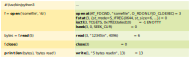
\includegraphics[width=\paperwidth]{../images/sample-listing.pdf}
  \end{columns}

\end{frame}

\begin{frame}[fragile]
  \frametitle{Fehlerfall}

  \begin{lstlisting}
% rm somefile
% strace notfound.py > output.txt
  \end{lstlisting}

  \begin{exampleblock}{\vspace*{-2ex}}
  \begin{lstlisting}
...
openat(AT_FDCWD, "somefile", O_RDONLY|O_CLOEXEC) =
   -1 ENOENT (Datei oder Verzeichnis nicht gefunden)
...
  \end{lstlisting}
  \end{exampleblock}


\end{frame}

\subsection{Kindprozesse und Threads}

\begin{frame}[fragile]
  \frametitle{Kindprozesse und Threads}

  \begin{block}{Prozesse und Threads}
    \begin{itemize}
      \item Kernel behandelt Threads und Prozesse erstmal ähnlich (als Scheduling-Einheit)
      \item Threads innerhalb des gleichen Prozesses haben gleiche PID aber andere TID
      \item \strace{} zeigt eigentlich die TID an, nennt das aber PID
     \end{itemize}
  \end{block}

  \begin{exampleblock}{Beispiel: \texttt{strace -f \ldots}}
    \begin{lstlisting}
clone(child_stack=0x7f4e991b0fb0, flags=CLONE_VM|CLONE_FS|CLONE_FILES|CLONE_SIGHAND|CLONE_THREAD|CLONE_SYSVSEM|CLONE_SETTLS|CLONE_PARENT_SETTID|CLONE_CHILD_CLEARTID, parent_tid=[40447], tls=0x7f4e991b1700, child_tidptr=0x7f4e991b19d0) = 40447
strace: Process 40447 attached
[pid 40447] set_robust_list(0x7f4e991b19e0, 24) = 0
[pid 40447] getpid()                    = 40446
          \end{lstlisting}
    \end{exampleblock}
\end{frame}

\subsection{Protokollierung in eine Datei}

\begin{frame}[fragile]
  \frametitle{Protokollierung in eine Datei}

  \vspace{-1mm}

  \begin{lstlisting}
    % strace -o DATEINAME
  \end{lstlisting}

  \vspace{-1mm}

  \begin{block}{Vorteile}
    \begin{itemize}
      \item Ausgabe von Programm und \strace{} klar getrennt
      \item Suchfunktion
      \item ggf. Syntax-Highlighting (vim)
     \end{itemize}
  \end{block}

  \begin{block}{Mehrere Prozesse}
    \begin{itemize}
      \item mit  Option \texttt{-ff} statt \texttt{-f}
         wird pro Kindprozess wird eigene Datei erstellt
      \item Namensschema \texttt{\emph{Dateiname.}PID}
     \end{itemize}
  \end{block}

  \begin{block}{Zeitstempel}
    \begin{itemize}
      \item \texttt{-t}: Sekunden-Genauigkeit
      \item \texttt{-tt}: Millisekunden-Genauigkeit
    \end{itemize}
  \end{block}
\end{frame}

\subsection{Filterfunktionen}

\begin{frame}[fragile]
  \frametitle{Filterfunktion: Einschränkung der Systemaufrufe}

  \begin{lstlisting}
    % strace -e trace=SET
    % strace -e trace=open,close # nur open und close
    % strace -e trace=%file      # Dateioperationen (Gruppe)
  \end{lstlisting}

  \begin{center}
    \begin{tabular}{|p{2cm}p{8.5cm}|}
      \hline
      \textbf{Gruppe} & \textbf{Operationen} \\
      \hline
      \texttt{\%file}          & Dateioperationen, die einen Dateinamen als Argument
                                bekommen, also beispielsweise \texttt{open,} \texttt{stat,}
                                \texttt{chmod,} \texttt{unlink,} … \\
      \texttt{\%desc}          & Dateioperationen, die einen Dateideskriptor als \newline
                                 Argument bekommen, also z.\,B. \texttt{read,} \texttt{write,}
                                \texttt{chmod,} \texttt{unlink,} … \\
      \texttt{\%process}       & Systemaurufe zur Prozessverwaltung \\
      \texttt{\%net}           & Systemaurufe zur Netzwerkprogrammierung \\
      \texttt{\%signal}        & Systemaurufe bzgl. Behandlung von Signalen \\
      \texttt{\%ipc}           & Operationen zur Interprozesskommunikation \\
      \texttt{\%memory}        & Systemaufrufe zur Speicherverwaltung \\
      \texttt{\%pure}          & Systemaufrufe ohne Argument, z.\,B. \texttt{getpid} \\
      \hline
    \end{tabular}
  \end{center}

\end{frame}

\begin{frame}[fragile]
  \frametitle{Filterfunktion: Erfolg oder Misserfolg}

  \begin{itemize}
    \item \texttt{-z} filtert nach erfolgreichen Systemaufrufen
    \item \texttt{-Z} filtert nach Systemaufrufen, die einen Fehlercode zurückliefern
  \end{itemize}
  
  \bigskip

  \begin{center}
    \includegraphics[width=8cm]{../images/success-failure.jpg}
  \end{center}

\end{frame}

\subsection{Strings (Zeichenketten)}

\begin{frame}[fragile]
  \frametitle{Strings}

  \begin{itemize}
    \item Strings werden standardmäßig ab 50 Zeichen abgeschnitten
    \item mit der Option \texttt{-s \emph{LÄNGE}} kann Limit erhöht werden
    \item Dateinamen werden immer vollständig ausgegeben
  \end{itemize}

\end{frame}


\subsection{\strace{} einschränken}


\subsection{Strings}

\section{Bereits laufende Prozesse}


\begin{frame}
  \frametitle{Laufende Prozesse}

  \begin{itemize}
    \item es können bereits laufende Prozesse verfolgt werden
    \item Tracing erst ab dem aktuellen Zeitpunkt, nicht „rückwirkend“
    \item Ermittlung der PID
      \begin{itemize}
        \item \texttt{pidof \emph{NAME}}
        \item \texttt{ps aux | grep \emph{NAME}}
      \end{itemize}
    \item Aufruf von \strace{}
      \begin{itemize}
        \item \texttt{strace -p \emph{PID} [-f]}
      \end{itemize}
  \end{itemize}
\end{frame}

\subsection{Konfiguration der Berechtigungen}

\begin{frame}[fragile]
  \frametitle{Konfiguration der Berechtigungen}

  \begin{block}{Wann ist \strace{} laufender Prozesse erlaubt?}
    \begin{itemize}
      \item Root darf alle Prozesse verfolgen
      \item Benutzer darf eigene Prozesse verfolgen
      \item Standardeinstellung vieler Linux-Distributionen verbietet letzteres
    \end{itemize}
  \end{block}

  \pause

  \begin{block}{Temporäres Freischalten}
    \texttt{sysctl kernel.yama.ptrace\_scope=0}
  \end{block}

  \begin{exampleblock}{Dauerhafte Konfiguration: /etc/sysctl.d/10-trace.conf}
    \texttt{kernel.yama.ptrace\_scope=0}
  \end{exampleblock}

\end{frame}

\subsection{Zuordnung von Dateideskriptoren}

\begin{frame}[fragile]
  \frametitle{Zuordnung von Dateideskriptoren}

  \begin{exampleblock}{\texttt{/proc/\emph{PID}/fd}}
    \begin{lstlisting}
lrwx------ 1 bw bw 64  2. Jan 16:35 0 -> /dev/pts/1
lrwx------ 1 bw bw 64  2. Jan 16:35 1 -> /dev/pts/1
lrwx------ 1 bw bw 64  2. Jan 16:35 2 -> /dev/pts/1
lr-x------ 1 bw bw 64  2. Jan 16:35 3 -> /home/bw/devel/strace-talk/sample/somefile
    \end{lstlisting}
  \end{exampleblock}

  \begin{block}{Automatische Zuordnung durch \strace{}}
    \texttt{strace -y}
  \end{block}

\end{frame}

{
  \usebackgroundtemplate{\includegraphics[height=1.0\paperheight]{../images/pinguine.pdf}}
  \begin{frame}[b,plain]
    \begin{mdframed}[tikzsetting={fill=white,fill opacity=0.9},backgroundcolor=none,leftmargin=0,
    leftmargin=40,rightmargin=40,skipbelow=80,innertopmargin=6mm,innerbottommargin=6mm]

    \begin{center}
      \emph{Vielen Dank für Eure Aufmerksamkeit!}
    \end{center}
  \end{mdframed}
  \vspace{2cm}

\end{frame}
}



\end{document}

% vim: set sw=2 ts=2 et tw=100: